% +------------------------------------------------------------------------+
% | CGAL Reference Manual:  Subdivision_surfaces_3
% +------------------------------------------------------------------------+
% | Subdivision surfaces on generic Polyhedron.
% | 
% | 1.2.2005  Le-Jeng Andy Shiue
% |
\RCSdef{\subdivisionRev}{$Revision$}
\RCSdefDate{\subdivisionDate}{$Date$}
% +------------------------------------------------------------------------+

\newcommand\DS{Doo-Sabin}

% ------------------------------------------------------------------------
\newcommand\FIGDIR{Subdivision_surfaces_3/FIG}
\newcommand\IL{{\itshape left}}
\newcommand\IR{{\itshape right}}
\newcommand\IM{{\itshape middle}}
\newcommand\IT{{\itshape top}}
\newcommand\IB{{\itshape bottom}}
% ------------------------------------------------------------------------

\ccParDims

\chapter{Subdivision Surfaces}
\label{chapterSubdivision}
\ccChapterRelease{\subdivisionRev. \ \subdivisionDate}
\ccChapterAuthor{Le-Jeng Andy Shiue}
\hspace{.4cm}
\begin{ccTexOnly}
    \setlength{\unitlength}{1mm}
    \begin{picture}(0,0)(0.0,0.0)
      \put (78,25){% textwidth = 156mm
          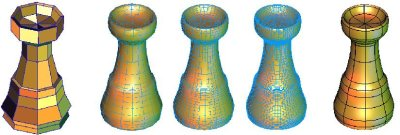
\includegraphics[width=0.45\textwidth]{\FIGDIR/QTSub}
      }
    \end{picture}\vspace{-4mm}% compensate for some vspace added by picture
\end{ccTexOnly}

\minitoc

% +------------------------------------------------------------------------+
\section{Introduction} \label{sectionSubIntro}
% +------------------------------------------------------------------------+
The subdivision algorithm is a simple yet powerful way to 
generate smooth surfaces from arbitrary polyhedral meshes. 
Unlike spline-based surfaces (e.g NURBS) or other numeric-based 
modeling techniques, users of subdivision
surfaces do not need in-depth mathematics 
knowledge on subdivision algorithms. An artist only need 
natural geometric intuitions to control the subdivision 
surfaces. It is hence especially popular for character 
modeling in video games and character animations.

%Subdivision algorithms (see e.g.~\cite{cgal:ww-smgd-02})
%recursively refine coarse meshes and generate ever closer 
%approximations to a smooth surface.
%for character animation, surface modeling, or physics simulation.
%Setting aside the specific strategy of geometric averaging
%for the new points, subdivision algorithms can be classified 
%according to the topological refinement of the underlying mesh.
%\ccc{Subdivision_surfaces_3}, working on the concept of the 
%\ccc{CGAL::Polyhedron_3} (see Chapter~\ref{chapterPolyhedron}),
%takes advantage of this separation of geometry and topology.
%Each subdivision algorithm is a refinement function parametrized
%by a set of rountines of geometric averageing.

While many subdivision schemes have been developed and new schemes 
are still being researched, \ccc{Subdivision_surfaces_3} 
supports the families of the four most used schemes: 
Loop, Catmull-Clark, Doo-Sabin and $\sqrt{3}$ subdivisions. 
\ccc{Subdivision_surfaces_3}, working on the concept of 
the \ccc{CGAL::Polyhedron_3} (see Chapter~\ref{chapterPolyhedron}), 
aims to be simple to use and powerful to extend.

\begin{ccHtmlOnly}
     <CENTER>
         <img src="./FIG/QTSub.jpg" alt="QT subdivision on a rook model"><P>
     </CENTER>
\end{ccHtmlOnly}

% +------------------------------------------------------------------------+
\section{Subdivision Algorithms}
\label{secSubAlgo}
% +------------------------------------------------------------------------+
In this chapter, we explain some fundamentals of 
subdivision surfaces. We only focus on the topics helping you 
to understand the design of the package; interested readers can
still refer to \cite{cgal:ww-smgd-02} for an in-depth introduction.
Some terminologies introduced in this section will be used again
in later sections. For users just want to use Loop (or 
Catmull-Clark ...etc) subdivision, Section \ref{secFirstSub} 
gives a quick tutorial on using these subdivisions.

Subdivision algorithms recursively refine coarse meshes and generate 
ever closer approximations to a smooth surface.
%Subdivision algorithms (see e.g.~\cite{cgal:ww-smgd-02}) 
%define surfaces as the limit
%of recursive refinement of a polyhedral mesh, called
%\emph{control mesh}. 
%The refinements generate mesh points 
%to be smoothed to approximate the limit surface.   
The chapter teaser shows a sequence of a subdivision on 
a chess model. 

Many refinement patterns are used in practice. 
\ccc{Subdivision_surfaces_3} supports the four most popular 
patterns, and each of them is used by Loop, 
Catmull-Clark\cite{cgal:cc-rgbss-78}, Doo-Sabin 
and $\sqrt{3}$ subdivision.  

\begin{ccTexOnly}
  \begin{center}
    \parbox{0.6\textwidth}{%
      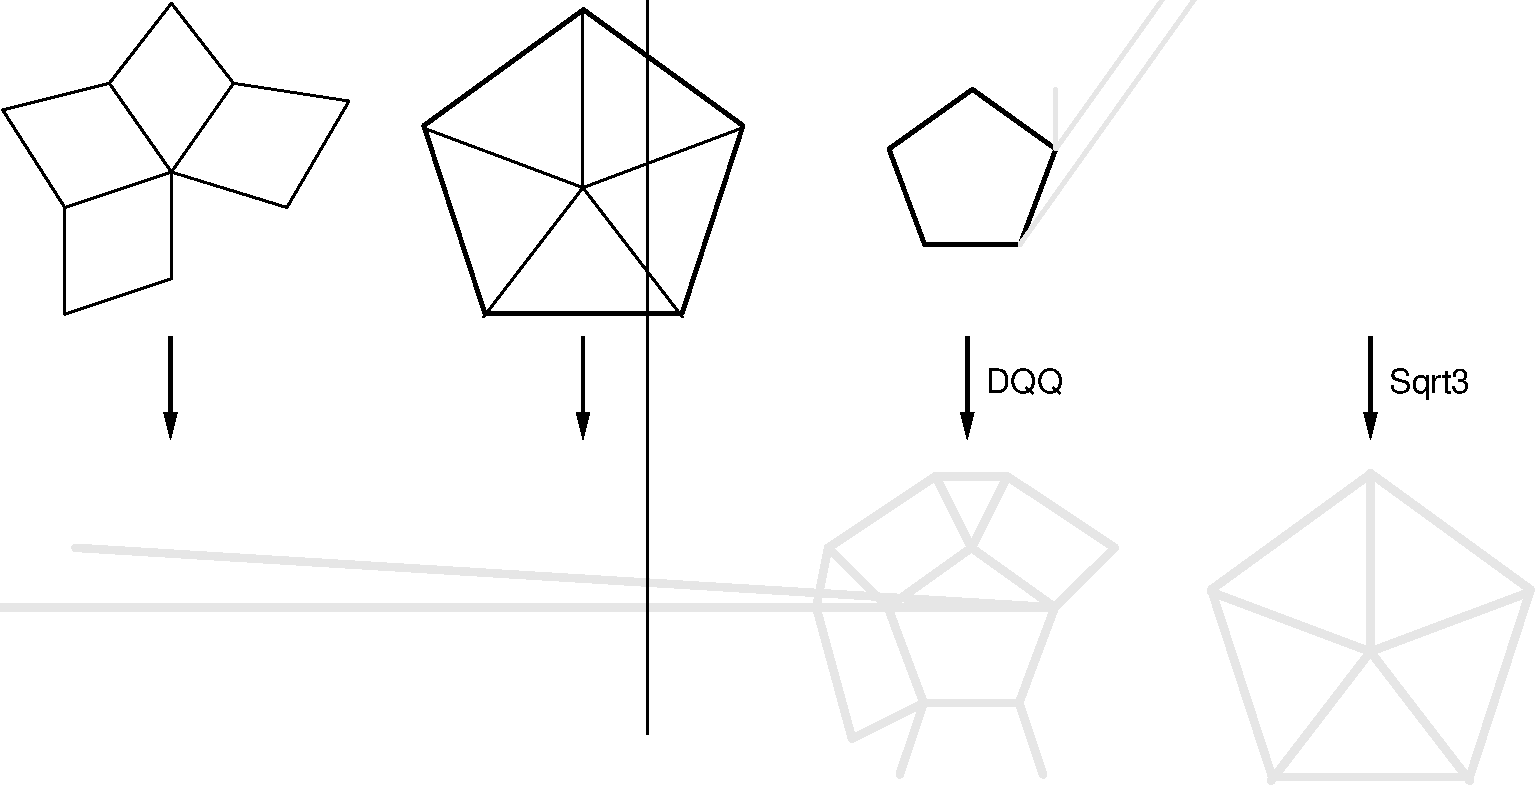
\includegraphics[width=0.6\textwidth]{\FIGDIR/RefSchemes}%
    }\\ \vspace{0.5cm}
  \end{center}
\end{ccTexOnly}

\begin{ccHtmlOnly}
  <CENTER>
     <img src="./FIG/RefSchemes.gif" alt="Refinement Hosts"><P>
  </CENTER>
\end{ccHtmlOnly}

Four refinement patterns are demonstrated on a valence-n mesh.
The refined mesh is shown below the input 
mesh (called \emph{control mesh}).
Points on the refined mesh are generated by averaging
neighbor points on the input mesh. A graph, called \emph{stencil}, 
determines the input submesh whose points contribute to the 
position of a refined point. A refinement pattern usually has 
several specific sets of stencils.
%Stencils are defined at the time the refinement pattern is chosen.  
%as illustrated in Figure \ref{fig:RefMap},
For example, the PQQ
%\emph{P}rimal \emph{Q}uadtrateral \emph{Q}uadrisection (PQQ) scheme 
refinement used by Catmull-Clark subdivision has a vertex-node stencil, 
which defines the 1-ring of an input vertex; an edge-node stencil, 
which defines the 1-ring of an input edge; and a facet-node stencil, 
which defines an input facet.

\begin{ccTexOnly}
  \begin{center}
    \parbox{0.5\textwidth}{%
      
\includegraphics[width=0.5\textwidth]{\FIGDIR/PQQStencil}%
    }\\ \vspace{0.5cm}
  \end{center}
\end{ccTexOnly}

\begin{ccHtmlOnly}
  <CENTER>
     <img src="./FIG/PQQStencil.gif" alt="Stencils of PQQ scheme "><P>
  </CENTER>
\end{ccHtmlOnly}


The blue neighborhoods in the top row indicate the corresponding
stencils of the refined nodes in red. 

%while the DQQ scheme has only a corner-node stencil, which 
%relates the facet of a corner to a target node.
Stencils with weights are called \emph{geometry masks}.
%One practical set of geometry masks of the PQQ scheme is
The geometric masks of Catmull-Clark subdivision are shown below.

\begin{ccTexOnly}
  \begin{center}
    \parbox{0.4\textwidth}{%
      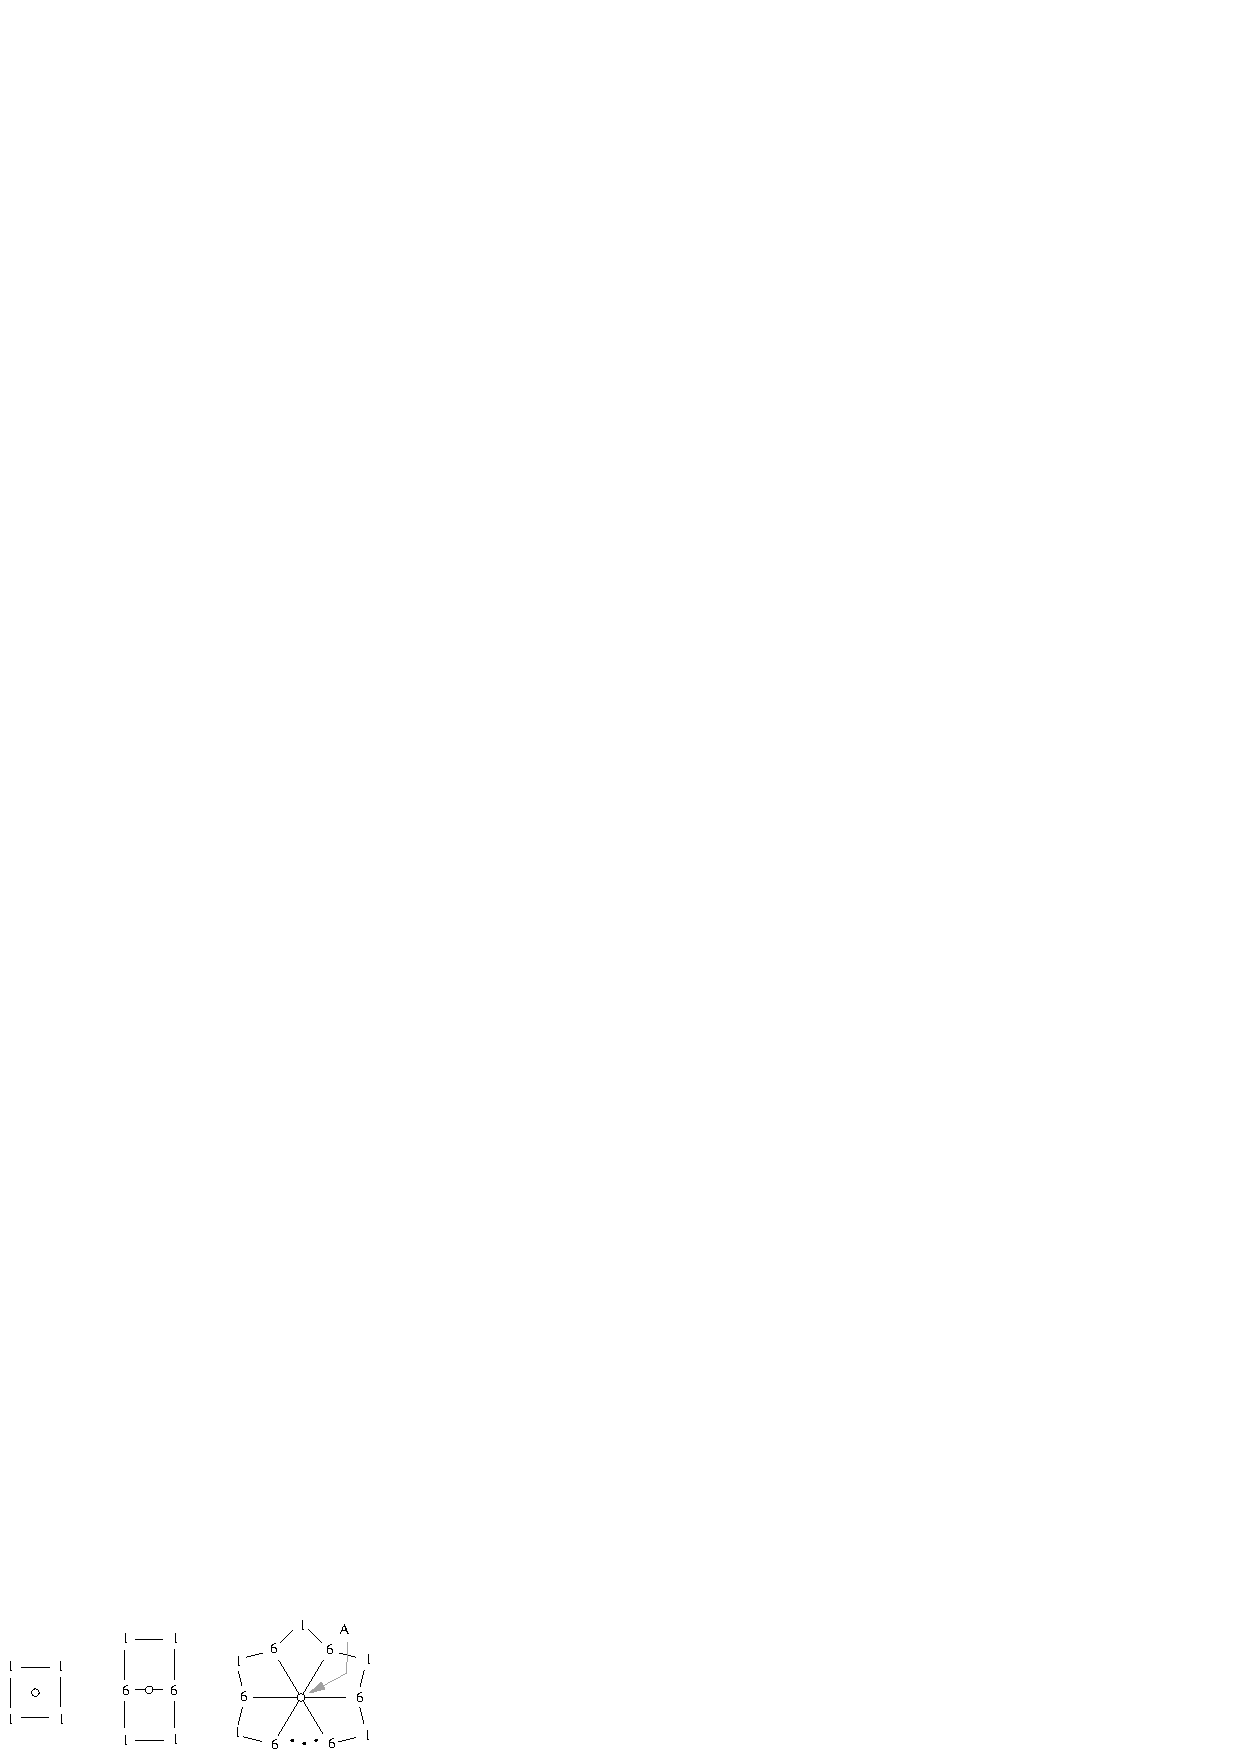
\includegraphics[width=0.4\textwidth]{\FIGDIR/cc_mask}%
    } \\ \vspace{0.5cm}
  \end{center}
\end{ccTexOnly}

\begin{ccHtmlOnly}
  <CENTER>
     <img src="./FIG/cc_mask.gif" alt="Catmull-Clark geometry stencil"><P>
  </CENTER>
\end{ccHtmlOnly}

The weights shown here are unnormalized, and $n$ is the valence 
of the vertex. The subdivided point, in red, is computed by a summation
of the weighted points on its stencil (i.e.~an input submesh).
For example, a Catmull-Clark facet-node is computed by the summation
of $1/4$ of each stencil node.

A stencil may have several specific sets of geometry masks. In other 
words, a facet-node of Catmull-Clark refinement may be computed by 
the summation of $1/5$ of each stencil node instead of $1/4$. 
Although it is legal in \ccc{Subdivision_surfaces_3} to have 
any kind of geometry mask, the result surfaces may be odd, 
not smooth, or not even exist.
To learn how to design a good mask, both mathematically and esthetically, 
readers can refer to \cite{cgal:ww-smgd-02}.

%The averaging process can typically be factored into 
%simpler steps \cite{Oswald-2003-CSS}.
%and this has been implemented in the OpenMesh library \cite{Sovakar-2004-APISUB}.
%However, while stencil factoring simplifies the implementation,
%it is less efficient because it requires repeated visits 
%to all nodes.

%% Since only a fixed number of refinement patterns are 
%% practical but a wide variety of geometry masks can be developed,
%% \ccc{Subdivision_surfaces_3} provides a set of refinement patterns 
%% (the \emph{refinement hosts})
%% and hands the definition of geometry masks
%% (the \emph{geometry policies}) to the library user.
%% A subdivision scheme is obtained by parameterizing the 
%% refinement host with geometry policies. 
%% For example, Catmull-Clark subdivision is constructed by 
%% parameterizing the PQQ refinement with the Catmull-Clark geometry 
%% policies.

%, which compute the smoothed points based on the
%Catmull-Clark geometry masks.

%A subdivision scheme of \ccc{CGAL::Subdivision_surfaces_3} is a 
%refinement host parameterized with a geometry policy. 

%The refinement host realizes the topological refinement and 
%the stencils. The geometry policy consists a set of 
%averaging rules of the geometry stencils.

% +-------------------------------------------------------------+
\section{Your First CGAL::Subdivision}
\label{secFirstSub}
Assuming that you already have a \emph{normal} CGAL polyhedral mesh,
say the default one, you can use the \ccc{Subdivision_surfaces_3}
without much effort.

\ccIncludeExampleCode{Subdivision_surfaces_3/CatmullClark_subdivision.C}

This example demonstrates the use of Catmull-Clark subdivision
on a read-in CGAL polyhedral mesh. There is only one line worth some
time to explain:
\begin{ccExampleCode}
Subdivision_surfaces_3<Polyhedron>::CatmullClark_subdivision(P,d);
\end{ccExampleCode}
\ccc{Subdivision_surfaces_3<Polyhedron>} defines a set of subdivision 
functions on the typename \ccc{Polyhedron}, and 
\ccc{CatmullClark_subdivision(P,d)} computes the 
Catmull-Clark subdivision surfaces of \ccc{d} steps from the 
\ccc{Polyhedron P}.

If you want to use Doo-Sabin subdivision instead, simply replace the 
\ccc{CatmullClark_subdivision(P,d)} to the \ccc{DooSabin_subdivision(P,d)}, 
and you are done. Note since Loop and $\sqrt{3}$ subdivision only work on 
triangle meshes, simply replacing the subdivision function may or 
may not work in this example as there is no assertion that a triangle 
mesh is read-in.

This example shows how to apply the subdivision algorithm 
on a simple \ccc{CGAL::Polyhedron_3}. When specializing the polyhedron,
there are two more things required to be kept in mind.  
First, the internal storage of your 
polyhedron has to be sequential ordered, such as the vector 
or the linked-list. A sequential ordered container always inserts new 
entries at the end. Secondly, typename \ccc{Point_3} is 
required to be defined within your polyhedron, otherwise our
subdivisions will not know how to compute and where to store the
new points. More details on these two requirements are explained
in Section~\ref{secRefHost}.

% +-------------------------------------------------------------+
\section{Catmull-Clark Subdivision in Depth}
\label{secCC}
In some situations, Loop, Catmull-Clark, Doo-Sabin and $\sqrt{3}$ 
subdivisions are just not the surfaces you would like to have. You 
may be a graduate student believing in a perfect subdivision scheme, or
you just want a unique surface which looks simply bad. In either case,
\ccc{Subdivision_surfaces_3} allows you to try your beloved algorithms
with a small amount of efforts. The best way to learn how to create
a your-name subdivision is by digging into one of the four subdivisions
\ccc{Subdivision_surfaces_3} supported. In this section, we will guide 
you through the creation of Catmull-Clark subdivision.
%This section explain how do we implement the
%Catmull-Clark subdivision based on the framework of 
%\ccc{Subdivision_surfaces_3}.

When a subdivision scheme is developed, a refinement scheme (i.e.~a 
parametrization) is chosen, and then a set of rules (i.e.~geometry 
masks) are developed to generate the new points (to meet certain 
mathematics conditions). E. Catmull and J. Clark picked the \emph{P}rimal 
\emph{Q}uadtrateral \emph{Q}uadrisection (PQQ) to be the refinement scheme,
and developed a set of geometry masks to generate (more precisely, to 
approximate) the B-spline surface from the input polyhedral mesh (i.e.~the 
control mesh). To implement Catmull-Clark subdivision, we need to 
implement the mesh data structure, the refinement on the mesh data 
structure, and the geometry masks. Luckily enough, we can use 
\ccc{CGAL::Polyhedron_3} as the mesh data structure, and use the 
PQQ function in \ccc{Subdivision_surfaces_3} to provide the refinement. 
\ccc{Subdivision_surfaces_3} also supports three other refinements that 
you can choose to use for your subdivision. These refinements are
PT(riangle)Q for Loop subdivision, D(ual)QQ for Doo-Sabin subdivision, 
and $\sqrt{3}$ triangulation for $\sqrt{3}$ 
subdivision. Here is the function declaration of the PQQ refinement.

\begin{ccExampleCode}
template <class Polyhedron>
class Subdivision_surfaces_3 {
  template <template <typename> class S>
  static void PQQ(Polyhedron& p, S<Polyhedron> rule, int step)
};
\end{ccExampleCode}

\ccc{Polyhedron} is a model of the \ccc{CGAL::Polyhedron_3}, and
\ccc{S} is a template class realizing geometry masks on the typename 
\ccc{Polyhedron}. \ccc{S} is called the
\emph{geometry policy} and \ccc{PQQ(...)} and other refinement 
functions are called the \emph{refinement hosts}. 
\ccc{step} specifies how many steps of the 
refinement are to be applied on the polyhedron \ccc{p}. To make the call to
\ccc{PQQ} a Catmull-Clark subdivision, the only thing left is to
implement a geometry policy realizing the Catmull-Clark geometry masks.

Before we can implement the Catmull-Clark geometry masks, we 
need to know the interfaces of these masks cooperated with
the refinement host. As we have already known, PQQ refinement has three
stencils. \ccc{Subdivision_surfaces_3} defines them as followings,
\begin{ccExampleCode}
template <class Polyhedron>
class PQQ_stencil_3 {
  void facet_node(Facet_handle facet, Point& pt) {}
  void edge_node(Halfedge_handle edge, Point& pt) {}
  void vertex_node(Vertex_handle vertex, Point& pt) {}
};
\end{ccExampleCode}

\ccc{PQQ_stencil_3} is a pure template interface and does nothing 
on generating points. It is our (or your) job to fill in the 
stencil functions with proper geometry masks. Lets compute the 
new points based on the Catmull-Clark geometry masks, and 
rename the policy to indicate geometry masks are in place.

\begin{ccExampleCode}
template <class Polyhedron>
class CatmullClark_mask_3 {
  void facet_node(Facet_handle facet, Point& pt) {
    Halfedge_around_facet_circulator hcir = facet->facet_begin();
    int n = 0;
    FT p[] = {0,0,0};
    do {
      Point t = hcir->vertex()->point();
      p[0] += t[0], p[1] += t[1], p[2] += t[2]; 
      ++n;
    } while (++hcir != facet->facet_begin());
    pt = Point(p[0]/n, p[1]/n, p[2]/n);
  }
  void edge_node(Halfedge_handle edge, Point& pt) {
    Point p1 = edge->vertex()->point();
    Point p2 = edge->opposite()->vertex()->point();
    Point f1, f2;
    facet_node(edge->facet(), f1);
    facet_node(edge->opposite()->facet(), f2);
    pt = Point((p1[0]+p2[0]+f1[0]+f2[0])/4,
               (p1[1]+p2[1]+f1[1]+f2[1])/4,
               (p1[2]+p2[2]+f1[2]+f2[2])/4 );
  }
  void vertex_node(Vertex_handle vertex, Point& pt) {
    Halfedge_around_vertex_circulator vcir = vertex->vertex_begin();
    int n = circulator_size(vcir);    

    float Q[] = {0.0, 0.0, 0.0}, R[] = {0.0, 0.0, 0.0};
    Point& S = vertex->point();
    
    Point q;
    for (int i = 0; i < n; i++, ++vcir) {
      Point& p2 = vcir->opposite()->vertex()->point();
      R[0] += (S[0]+p2[0])/2;
      R[1] += (S[1]+p2[1])/2;
      R[2] += (S[2]+p2[2])/2;
      facet_node(vcir->facet(), q);
      Q[0] += q[0];      
      Q[1] += q[1];      
      Q[2] += q[2];
    }
    R[0] /= n;    R[1] /= n;    R[2] /= n;
    Q[0] /= n;    Q[1] /= n;    Q[2] /= n;
      
    pt = Point((Q[0] + 2*R[0] + S[0]*(n-3))/n,
               (Q[1] + 2*R[1] + S[1]*(n-3))/n,
               (Q[2] + 2*R[2] + S[2]*(n-3))/n );
  }
};
\end{ccExampleCode}

Now, we are ready to make our first call of Catmull-Clark 
subdivision.

\begin{ccExampleCode}
template <class Polyhedron>
class Subdivision_surfaces_3 {
  void CatmullClark_subdivision(Polyhedron& p, int step) {
    PQQ(p, CatmullClark_mask_3<Polyhedron>(), step);
  }
}
\end{ccExampleCode}

Loop, Doo-Sabin and $\sqrt{3}$ subdivisions are all created in the
same way, but with different combinations of the 
refinement host and the geometry policy. For you to be able to 
develop your own subdivision, you need to know how to choose the 
right combination and how to combine them within the framework
of \ccc{Subdivision_surfaces_3}. This is explained in the next section.

% +-------------------------------------------------------------+
\section{Refinement Host}
\label{secRefHost}
\ccc{Subdivision_surfaces_3} provides four refinement hosts of primal 
quadrilateral quadrisection (PQQ), primal triangle 
quadrisection (PTQ), dual quadrilateral 
quadrisection (DQQ) and $\sqrt{3}$ triangulation, which 
are used by Catmull-Clark, Loop, \DS\ and $\sqrt{3}$ subdivision, 
respectively. 

\begin{ccTexOnly}
  \begin{center}
    \parbox{0.6\textwidth}{%
      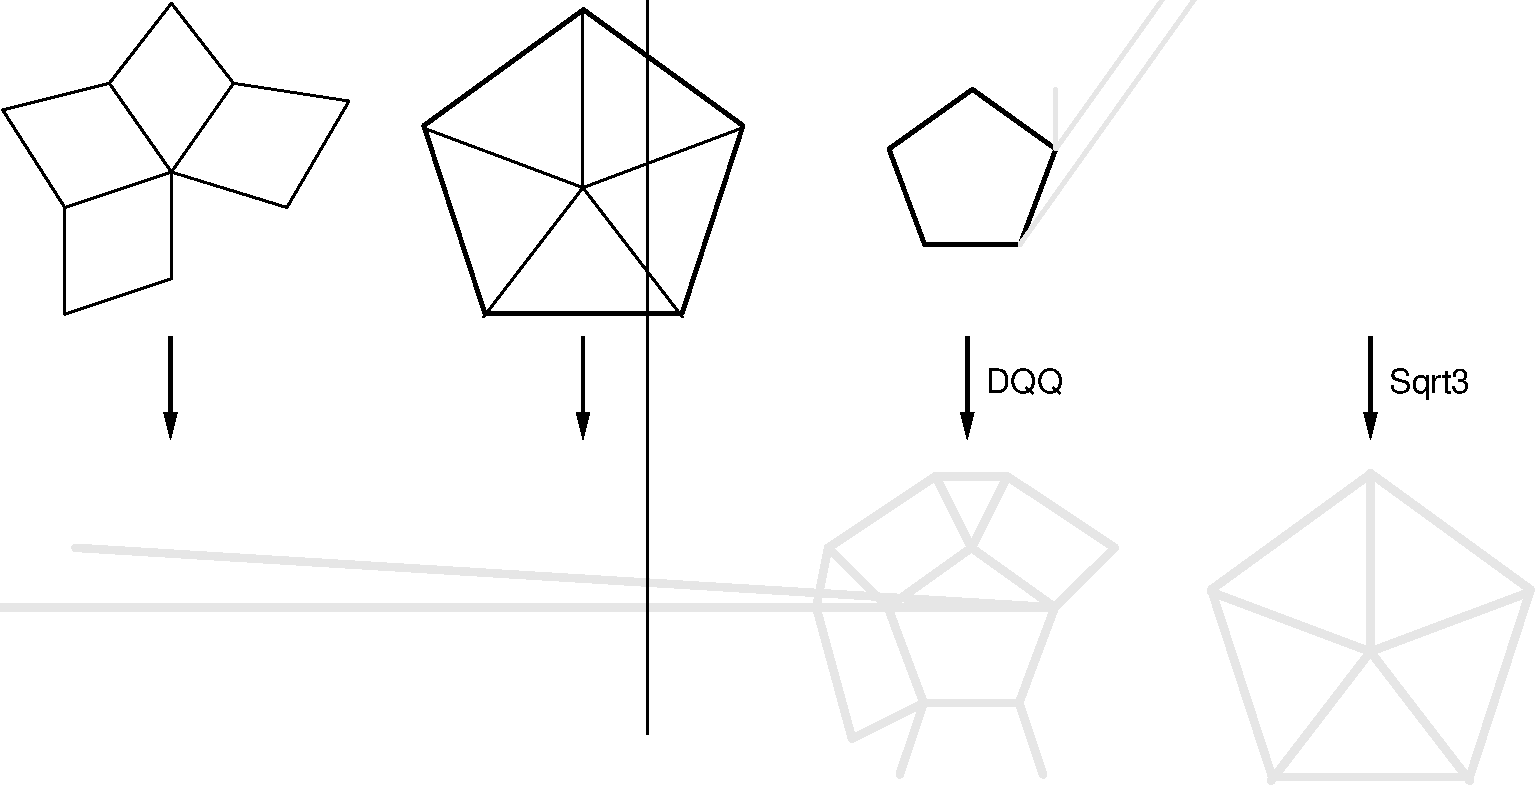
\includegraphics[width=0.6\textwidth]{\FIGDIR/RefSchemes}%
    }\\ \vspace{0.5cm}
%    \ccc{Subdivision_surfaces_3} supports hosts of these four refinement 
%    schemes that are demonstrated on a valence-n submesh.
%    The refined mesh is shown below the control mesh.
  \end{center}
\end{ccTexOnly}

\begin{ccHtmlOnly}
  <CENTER>
     <img src="./FIG/RefSchemes.gif" alt="Refinement Hosts"><P>
  </CENTER>
\end{ccHtmlOnly}


\begin{ccExampleCode}
template <class Polyhedron>
class Subdivision_surfaces_3 {
  // S is the geometry policy realizing the geometry masks
  template <template <typename> class S>
  static void PQQ(Polyhedron& p, S<Polyhedron> rule, int step);

  template <template <typename> class S>
  static void PTQ(Polyhedron& p, S<Polyhedron> rule, int step);

  template <template <typename> class S>
  static void DQQ(Polyhedron& p, S<Polyhedron> rule, int step);

  template <template <typename> class S>
  static void Sqrt3(Polyhedron& p, S<Polyhedron> rule, int step);
}
\end{ccExampleCode}

%% Stencils are maintained using the iteration concept
%% to avoid the need for vertex tags to distinguish
%% the stencil types.
%% For example, on a PQQ refined mesh, the vertex iterator 
%% visits the 
%% vertex-nodes, edge-nodes and then facet-nodes. The visit
%% order is implicitly used to determine the stencil of
%% the visited node.

Each refinement host is a template function of
a polyhedron type and a policy type. The polyhedron type is
a model of the \ccc{CGAL::Polyhedron_3} concept, and the
policy type is a class with functions realizing the 
geometry masks of a specific subdivision scheme.

Refinement hosts refine the polyhedron, maintain the stencils 
(i.e.~the mapping between the control mesh and the refined mesh), 
and call policy functions to compute and assign the new points. 
In our implementation, refinements are done by applying a 
sequence of connectivity operations (mostly Euler operations).
The stencils are maintained by ordering nodes on the refined 
polyhedron to match the sequence of the connectivity operations. 
By matching the order, no flag to classify the stencils 
is required to maintain and access the stencils.
But to make the ordering trick work, the polyhedron type need 
to use an internal storage with sequential ordering, such as
a vector or a linked-list. A sequential ordered container inserts
new entries at the end, and its iterator visits the entries in the 
order of their insertion. Non-sequential structures such as 
tree or map do not provide the required ordering, and hence
can not be used with \ccc{Subdivision_surfaces_3}.
 
Although \ccc{Subdivision_surfaces_3} does not require flags or 
tags to support the refinements and the stencil accesses, it
still need to know how to compute and where to store the geometry
data (in most cases, the points). \ccc{Subdivision_surfaces_3} 
expects that the typename \ccc{Point_3} is 
defined in the scope of \ccc{Polyhedron} and \ccc{Polyhedron::Vertex}. 
The refinement hosts use
this point type as the geometry holder and delegate the geometry
computation to the geometry policies. The geometry policy is 
explained in next section. 

For details of the refinement algorithm and implementation, 
interested users can refer to \cite{cgal:sp-mrbee-05}.

% +-------------------------------------------------------------+
\section{Geometry Policy}
A geometry policy defines a set of geometry masks. 
Each geometry mask is realized as a member function (i.e.~the 
policy function) computing and assigning new points according 
to a particular subdivision scheme. 
%The policy interface is defined with the refinement host. 

Each policy function receives a primitive handle 
(e.g.~\ccc{Halfedge_handle}) of the control polyhedron, 
and the reference of the \ccc{Point} to the refined vertex. 
In general, the implementation of the policy function 
collects the neighbors of the primitive handle (i.e.~nodes 
on the stencil), and (ideally) computes the new point 
by a linear combination of the stencil 
nodes and the mask (i.e.~the stencil weights).

\begin{ccTexOnly}
  \begin{center}
    \parbox{0.4\textwidth}{%
      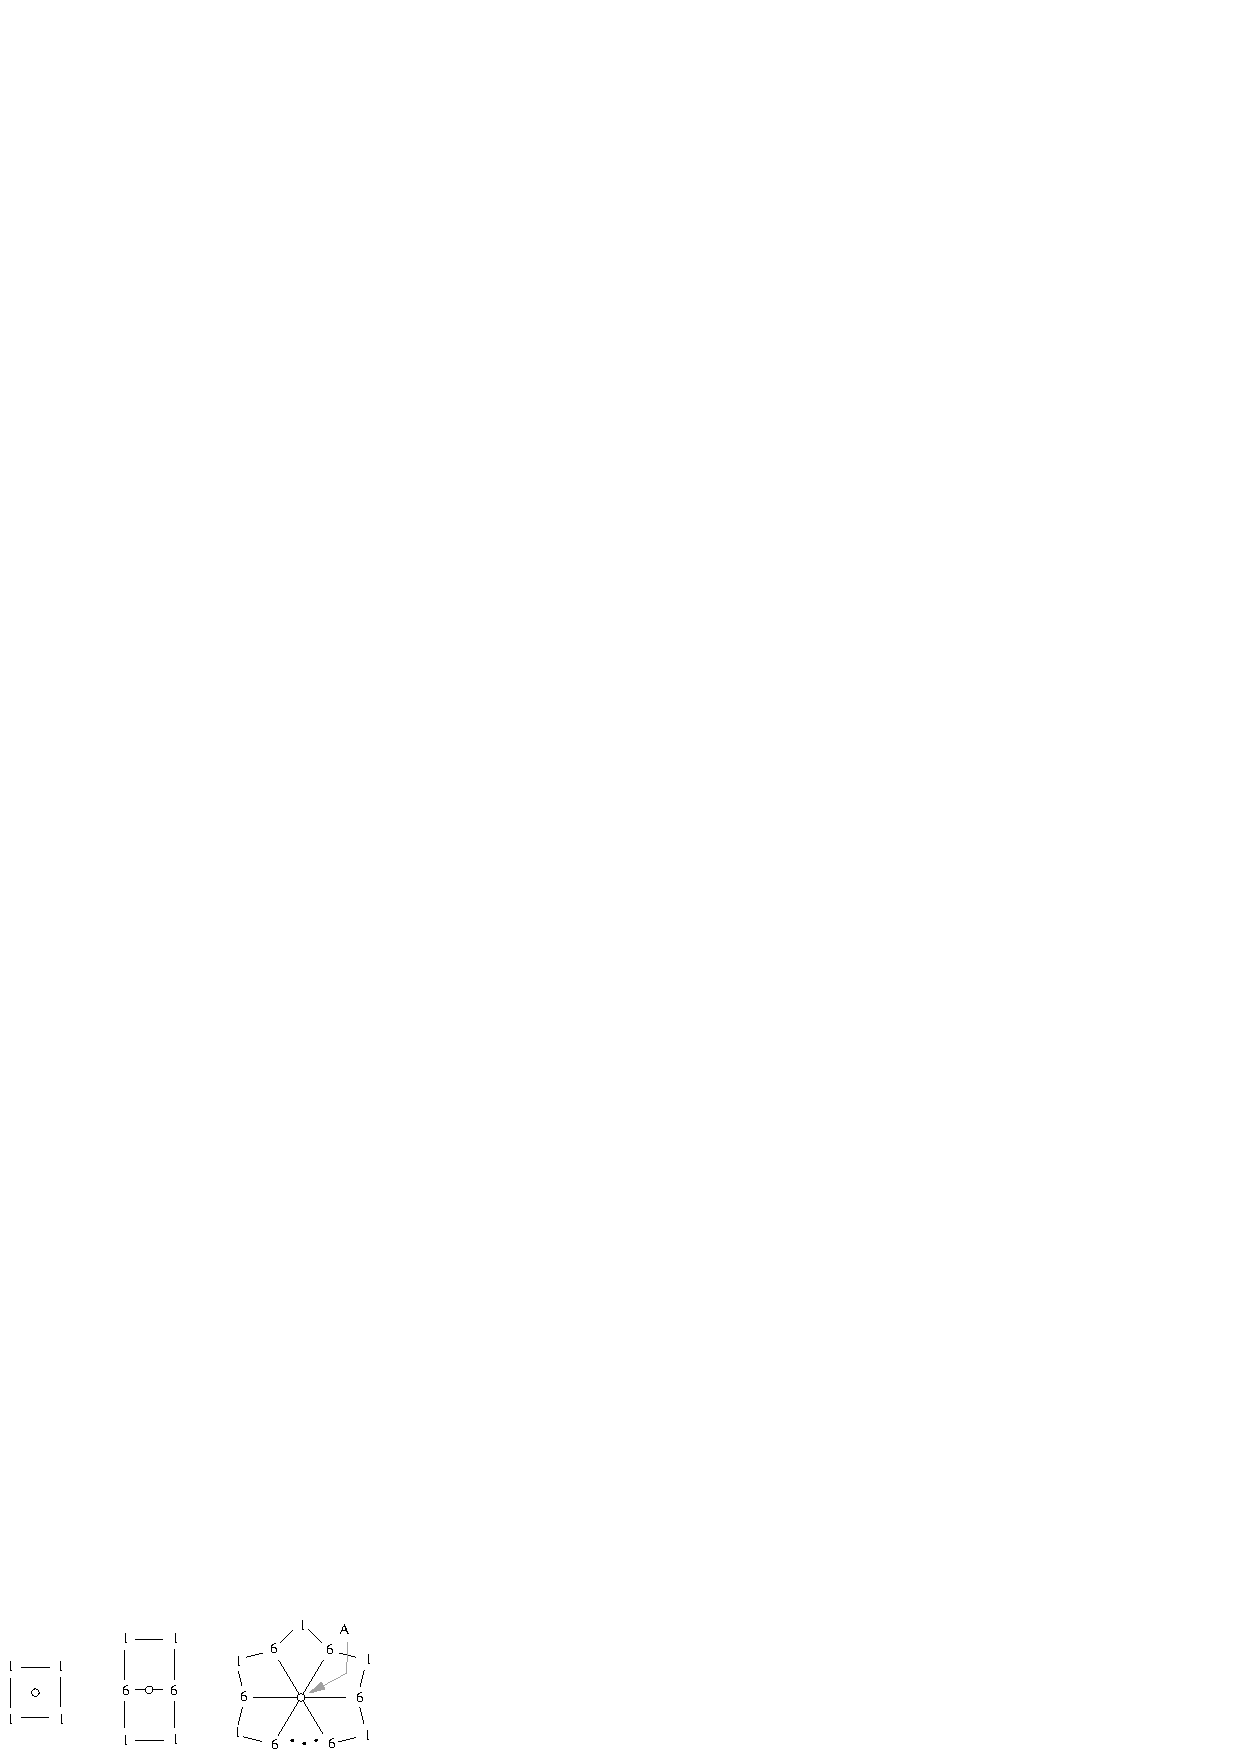
\includegraphics[width=0.4\textwidth]{\FIGDIR/cc_mask}%
    } \\ \vspace{0.5cm}
  \end{center}
\end{ccTexOnly}
\begin{ccHtmlOnly}
  <CENTER>
     <img src="./FIG/cc_mask.gif" alt="Catmull-Clark geometry stencil"><P>
  </CENTER>
\end{ccHtmlOnly}

This picture shows the stencils and the geometry masks for
Catmull-Clark subdivision. The weights shown here are unnormalized, 
and $n$ is the valence of the vertex. The new points are 
computed by the summation of the weighted points on their stencils.
Following codes show an implementation of the geometry policy of 
the facet-node. \ccc{Point} is a typedef to the \ccc{Point_3}
in \ccc{Polyhedron}. Note when \ccc{n} is $4$, this policy computes 
the facet-node shown in the above picture. The complete listing
of the Catmull-Clark policy class is in the Section~\ref{secCC}.

\begin{ccExampleCode}
template <class Polyhedron>
class CatmullClark_mask_3 {
  void facet_node(Facet_handle facet, Point& pt) {
    Halfedge_around_facet_circulator hcir = facet->facet_begin();
    int n = 0;
    FT p[] = {0,0,0};
    do {
      Point t = hcir->vertex()->point();
      p[0] += t[0], p[1] += t[1], p[2] += t[2]; 
      ++n;
    } while (++hcir != facet->facet_begin());
    pt = Point(p[0]/n, p[1]/n, p[2]/n);
  }
}
\end{ccExampleCode}

In this example, \ccc{Point} is assumed to be a \ccc{CGAL::Point_3}.
But you are allowed to use any point \emph{type} as long as it is type
defined as \ccc{Point_3} in your polyhedron class and vertex class.
You may need to modify the geometry policy to support the computation
and assignment of your specialized point. This extension is not unusual 
in graphics applications. For example, you might want to subdivide the
texture coordinates when you subdivide the polyhedron. The typename 
\ccc{Point_3} is actually the attribute holder, including the 
point of course, for the vertices.

The PQQ refinement host requires three policy functions for 
polyhedrons without open boundaries: a vertex-node 
stencil, an edge-node stencil, and a facet-node stencil. 
To support polyhedrons with boundaries, a policy function
for border vertices is also required. The border policy for
Catmull-Clark is given below.

%% \begin{ccTexOnly}
%%   \begin{center}
%%     \parbox{0.5\textwidth}{%
%%       
\includegraphics[width=0.5\textwidth]{\FIGDIR/PQQStencil}%
%%     }
%%   \end{center}
%% \end{ccTexOnly}

\begin{ccExampleCode}
  void border_node(Halfedge_handle edge, Point& ept, Point& vpt) {
    Point& ep1 = edge->vertex()->point();
    Point& ep2 = edge->opposite()->vertex()->point();
    ept = Point((ep1[0]+ep2[0])/2, (ep1[1]+ep2[1])/2, (ep1[2]+ep2[2])/2);

    Halfedge_around_vertex_circulator vcir = edge->vertex_begin();
    Point& vp1  = vcir->opposite()->vertex()->point();
    Point& vp0  = vcir->vertex()->point();
    Point& vp_1 = (--vcir)->opposite()->vertex()->point();
    vpt = Point((vp_1[0] + 6*vp0[0] + vp1[0])/8,
                (vp_1[1] + 6*vp0[1] + vp1[1])/8,
                (vp_1[2] + 6*vp0[2] + vp1[2])/8 );
  }
\end{ccExampleCode}


The interfaces of a geometry policy need to match the stencils of 
the refinement host. We have already seen the geometry masks for
a PQQ-base subdivision, Catmull-Clark subdivision, which gives
four stencil interfaces. The stencil interface the other three 
refinement host, PTQ, DQQ and $\sqrt{3}$, are defined below 
(PQQ as well).


\begin{ccExampleCode}
template <class Poly>
class PQQ_stencil_3 {
  void facet_node(Facet_handle, Point&) {};
  void edge_node(Halfedge_handle, Point&) {};
  void vertex_node(Vertex_handle, Point&) {};

  void border_node(Halfedge_handle, Point&, Point&) {};
};

template <class Poly>
class PTQ_stencil_3 {
  void edge_node(Halfedge_handle, Point&) {};
  void vertex_node(Vertex_handle, Point&) {};

  void border_node(Halfedge_handle, Point&, Point&) {};
};

template <class Poly>
class DQQ_stencil_3 {
public:
  void corner_node(Halfedge_handle edge, Point& pt) {};
};

template <class Poly>
class Sqrt3_stencil_3 {
public:
  void vertex_node(Vertex_handle vertex, Point& pt) {}
};
\end{ccExampleCode}

Note, only the \ccc{PQQ_stencil_3} and the \ccc{DQQ_stencil_3}
are provided in \ccc{Subdivision_surfaces_3}.
The \ccc{PTQ_stencil_3} and the \ccc{Sqrt3_stencil_3} are given
here for reference only. Both stencils are a subset of the
\ccc{PQQ_stencil_3}, and you can just use the 
\ccc{PQQ_stencil_3} to develop masks for PTQ or $\sqrt{3}$ 
schemes. Our DQQ and $\sqrt{3}$ refinement hosts do
not support global boundaries yet, hence the
\ccc{DQQ_stencil_3} and the \ccc{Sqrt3_stencil_3} do not
have the border-node policy (this might be changed in the 
future release). 


%% \begin{ccExampleCode}
%% PQQ<_M,CCstencil>(Mesh,CCstencil<_M>())
%% \end{ccExampleCode}
%% (or, more simply \\
%% \begin{ccExampleCode}
%% PQQ(Mesh,CCstencil<_M>())}
%% \end{ccExampleCode}
%% since the compiler can derive the template
%% arguments from the function parameters),
%% instantiates Catmull-Clark subdivision.    
%% \ccc{_M}, the model of the mesh concept,
%% represents the mesh type (\ccc{Mesh}),
%% and \ccc{CCstencil} is a class template 
%% realizing geometry policies of Catmull-Clark subdivision.

%The geometry stencils of Catmull-Clark subdivision (border stencils are 
%not included) are shown below. 

%\begin{ccTexOnly}
%  \begin{center}
%    \parbox{0.4\textwidth}{%
%      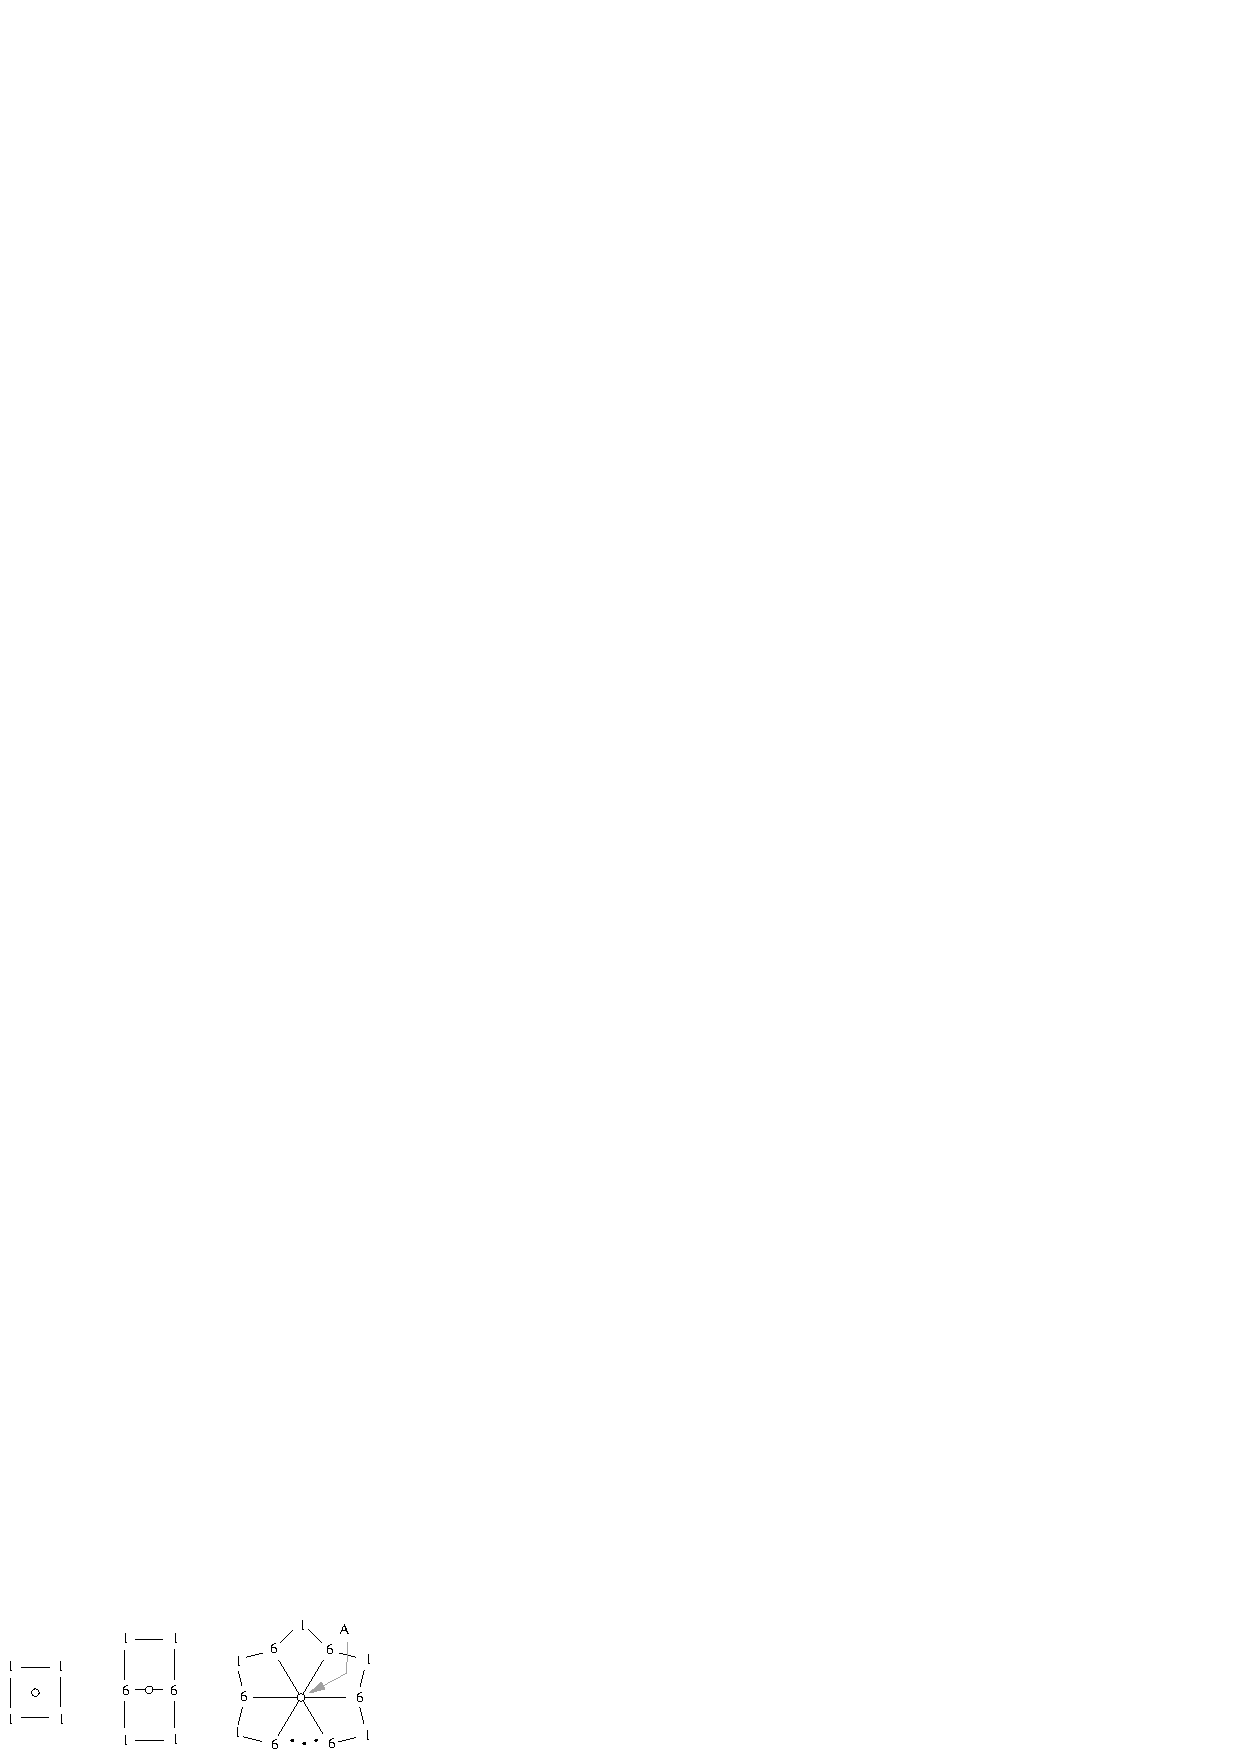
\includegraphics[width=0.4\textwidth]{\FIGDIR/cc_mask}%
%    }
%  \end{center}
%\end{ccTexOnly}

%\begin{ccHtmlOnly}
%  <CENTER>
%  <A HREF="./FIG/cc_mask.gif">
%     <img src="./FIG/cc_mask.gif" alt="Catmull-Clark geometry stencil"></A><P>
%  </CENTER>
%\end{ccHtmlOnly}


% +------------------------------------------------------------------------+
\section{Built-in subdivision schemes}
% +------------------------------------------------------------------------+
Considering their popularity in graphics modeling, 
Catmull-Clark, Loop, \DS\ and $\sqrt{3}$ subdivisions are directly
supported in \ccc{Subdivision_surfaces_3}. 
%Each of these subdivision schemes is realized by parameterizing 
%the corresponding geometry policy to the .

\begin{ccExampleCode}
  static void CatmullClark_subdivision(Polyhedron& p, int step) {
    PQQ(p, CatmullClark_stencil_3<Polyhedron>(), step);
  }
  static void Loop_subdivision(Polyhedron& p, int step) {
    PTQ(p, Loop_stencil_3<Polyhedron>() , step);
  }
  static void DooSabin_subdivision(Polyhedron& p, int step) {
    DQQ(p, DooSabin_stencil_3<Polyhedron>(), step);
  }
  static void Sqrt3_subdivision(Polyhedron& p, int step) {
    Sqrt3(p, Sqrt3_stencil_3<Polyhedron>(), step);
  }
\end{ccExampleCode}

The following shows an example of \DS\ subdivision on a polyhedral mesh.
\ccIncludeExampleCode{Subdivision_surfaces_3/DooSabin_subdivision.C}

% +------------------------------------------------------------------------+
\section{Customize subdivision schemes}
% +------------------------------------------------------------------------+
One of the goals of \ccc{Subdivision_surfaces_3} is 
to provide a flexible platform
to develop user-flavored subdivision schemes.
To construct a customized subdivision scheme, users can simply 
choose a refinement host with the intended topological pattern, 
and then realize the geometry policy accordingly. 
The following example develops a subdivision scheme
generating improved Loop subdivision surfaces. Loop subdivision is
based on PTQ refinement. The geometry policy is developed as a subclass 
of \ccc{PQQ_stencil_3}, which defines the superset of PTQ stencils.

\ccIncludeExampleCode{Subdivision_surfaces_3/Customized_subdivision.C}

A policy function for subdivision surfaces assigns a point on 
the subdivided polyhedron. The points are semantically
required to converge to a smoothed surface of the control mesh.
This is the text-book requirement of a subdivision 
surface (it has to be smooth). Since this is the end of the
class, feel free to throw the text-book away and just try yours. 
Good luck though.

